\subsection{Finite State Machine (Yang)}
A finite state machine with five states is used to determine where and what customized code segment should be injected into the original assembly program, shown in Figure \ref{fig:state_machine}.
\begin{figure}
\centering
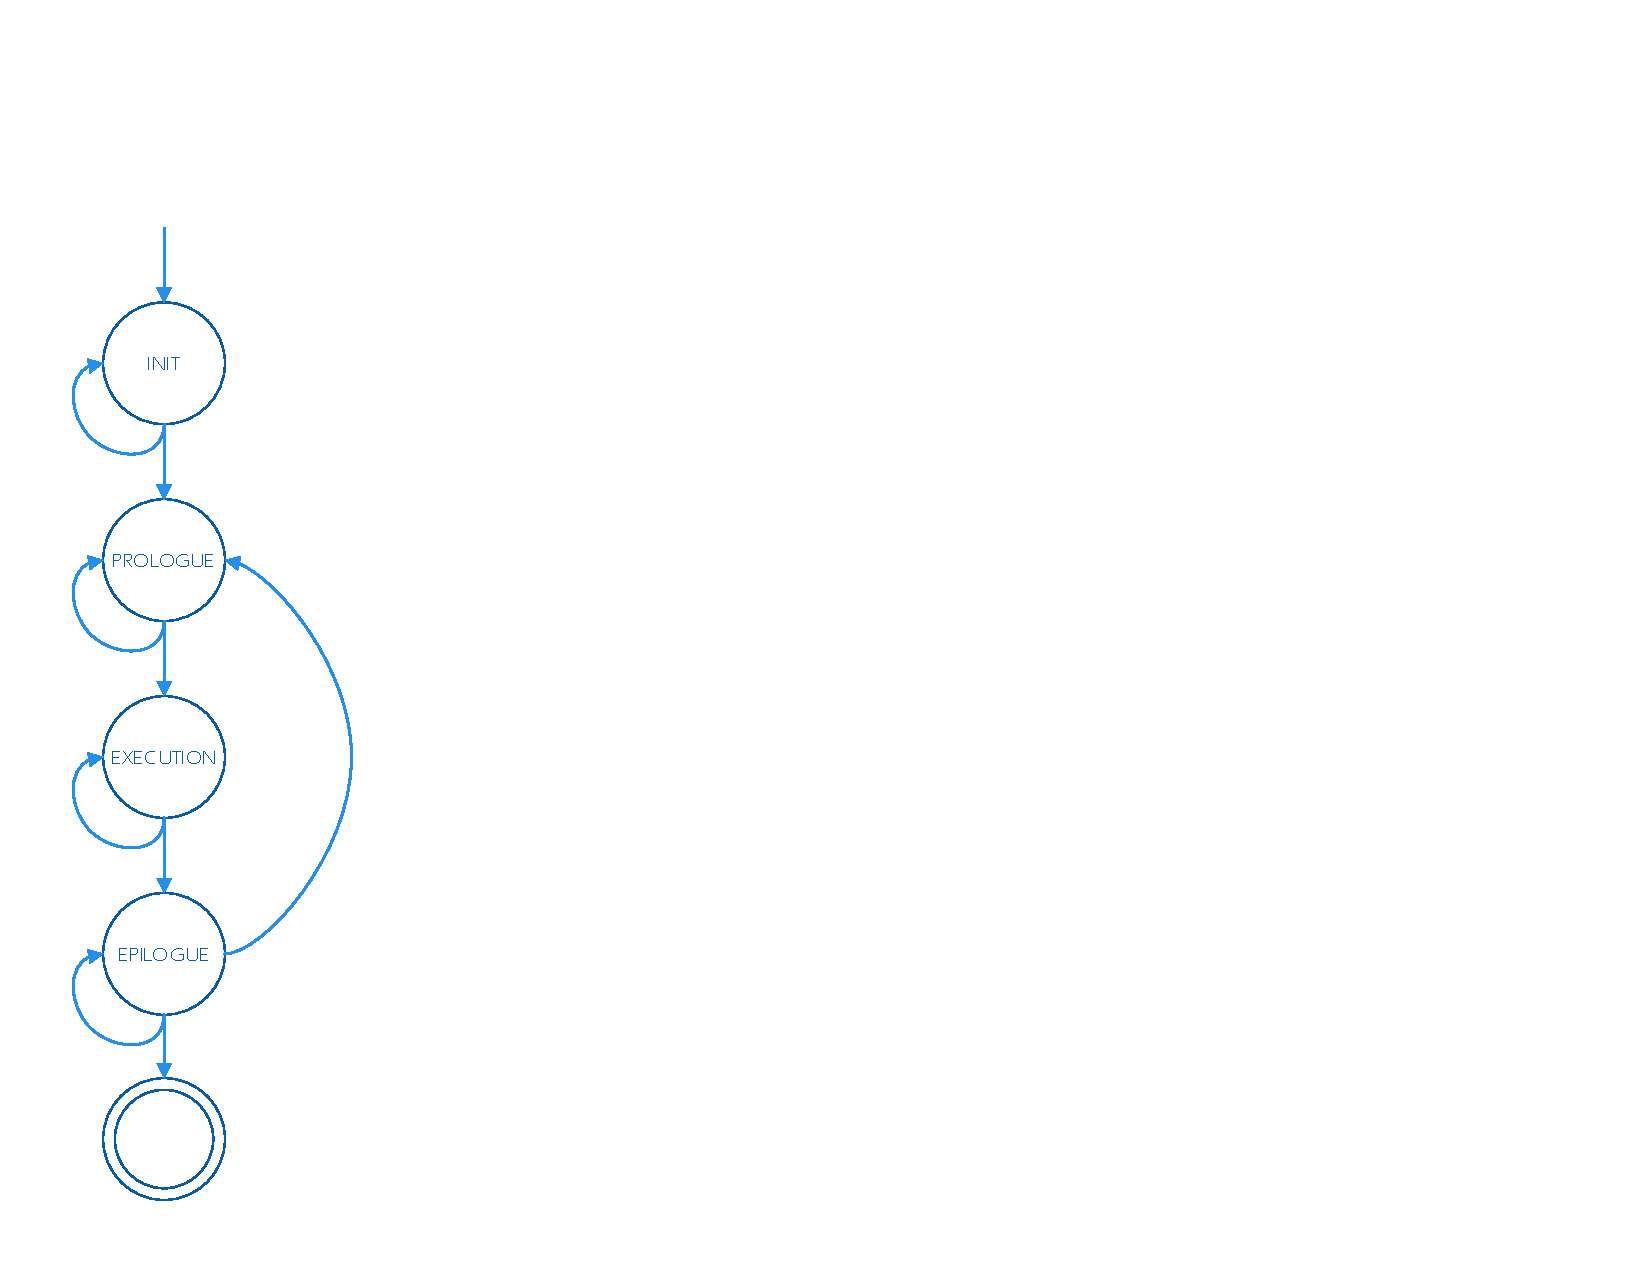
\includegraphics[scale=0.45]{figures/state_machine.pdf}
\caption{Finite State Machine}
\label{fig:state_machine}
\end{figure}

\subsubsection{INIT} 
\textit{INIT} is the start state of the finite state machine where the assembly program defines macros, global variables, and performs initialization operations such as xxx. The finite state machine will remain in \textit{INIT} state until the declaration of a new function, for example, ".global foo", is detected. A code segment which initializes the \textbf{SFS} and \textbf{STP} sections will be introduced before the state machine shifts its state to \textit{PROLOGUE}.

\subsubsection{PROLOGUE} 
\textit{PROLOGUE} is the state where a function backs up conflict registers and allocates space for stack frame. In this state, if "sbiw r28,\textit{n}" is scanned, the result of \textit{n} added by 6 will be stored as the size of the modified stack frame for later use.  The finite state machine will remain in \textit{PROLOGUE} state until the end of the function prologue, "out \_\_SP\_L\_\_,r28", is detected. A code segment which pushes the size of he modified stack frame to the stack will be introduced below this line. And if the function being processed currently is not the \textit{main} function, a code segment which calculates the CRC of the caller function, copys the contents in the stack, and updates the \textbf{SFS} and \textbf{STP} sections will also be introduced before the finite state machine shifts its state to \textit{EXECUTION}.

\subsubsection{EXECUTION} 
\textit{EXECUTION} is the state where a function finishes its main feature. The finite state machine will remain in \textit{EXECUTION} state until the beginning of the epilogue, "adiw r28,\textit{n}", is detected.  No additional code will be introduced before the finite state machine shifts its state to \textit{EPILOGUE}.

\subsubsection{EPILOGUE}
\textit{EPILOGUE} is the state where a function recovers the conflict registers and the stack. A code segment which calculates the CRC, compares the newly-calculated CRC with the CRC stored in stack, recovers the memory and updates the SFS and STP information will be introduced above the line "ret". The finite state machine will remain in \textit{EPILOGUE} state until the last line of the function epilogue, fox example, ".size	\textit{foo}, .-\textit{foo}", is detected. If there is no new line afterwards, the finite state machine will shift to the final state. Otherwise, the finite state machine will shift back to \textit{PROLOGUE} state.